% !TeX root = ../index.tex
\chapter{Design and Architecture}
\label{Proof of Latency}
\begin{figure}
	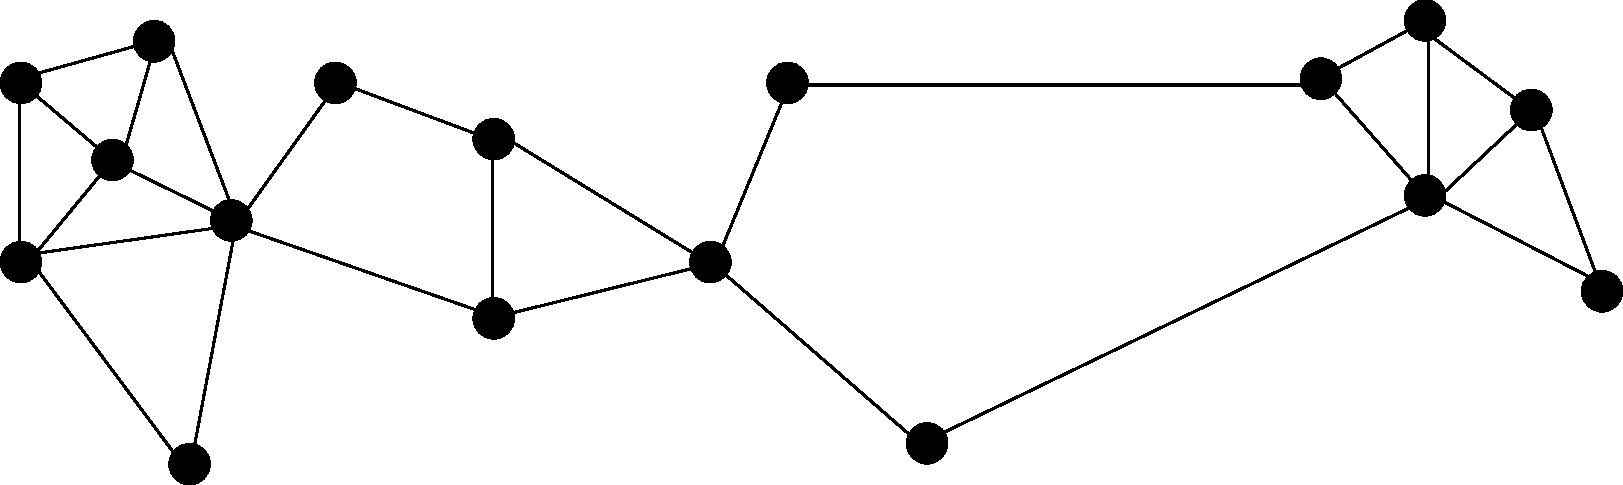
\includegraphics[width=\textwidth]{pictures/pol_topology.pdf}
	\caption{Example PoL network topology. Localized and highly connected clusters with high performance bridges, resulting in optimal routing}
	\label{PoL Example Topology}
\end{figure}
% TODO: Add a Figma-drawed image overarching the whole protocol, not just the distance bounding part
Proof of Latency, "the protocol" or "PoL", is a protocol that when used in a P2P context, can offer a way of reducing network latency between peers by connecting with peers that have the lowest latency between each other, thus establishing a more optimal network than achieved simply by peering at random. PoL aims to make network bootstrapping better, making it easier to find performant, physically close-by peers on the first interaction with a PoL-enabled network. When using PoL for peer discovery, it can result in a network in which a peer can at least roughly estimate its latency to another peer before connecting to it.

Distance bounding protocols, as previously described, are a way of measuring latency between two participants in a relatively unspoofable manner. Unfortunately, they can only provide a valid proof between the prover and the verifier, and not a third party. This is because a distance bound could have been calculated at any point in the past, and the prover and the verifier could quite easily craft a proof of 0 latency between them. The motivation for PoL was to try to fix this with its use of verifiable delay functions, but further research revealed that some additional logic was needed to cater to a decentralized setting.

The protocol is trustless between the two computing parties and it requires no specific hardware from the participants. This said, special hardware for speeding up its evaluation and proving could make it a better protocol at distance bounding, as difference in the processing powers cause measurement error.

Aside from constructing P2P networks with better routes, the protocol could be used as a benchmark query or a proof of geographical location. A proof of a geographical location could prove useful, since GPS coordinates along with IP addresses can be spoofed.

\section{Protocol Description}
\begin{table}[h!]
	\centering
	\begin{tabular}{ c|c  }
		Symbol        & Description                                             \\
		\hline
		\( p \)       & Prover                                                  \\
		\( v \)       & Verifier                                                \\
		\( \lambda \) & Processing power                                        \\
		\( c \)       & Vector commitment                                       \\
		\( N \)       & The modulus used in a VDF. \(RSA-2048\)~in this context.   \\

		\( T \)       & The difficulty of a VDF (the number of squarings)       \\
		\( g \)       & The generator of a VDF. Formally, \(c_p c_v\).          \\
		\( l \)       & A random prime number                                   \\
		\( VDF \)     & A verifiable delay function                             \\
		\( x \)       & The result of a VDF                                     \\
		\(\pi \)      & The proof of a VDF                                      \\
		\(\Delta\)    & The measured latency. Formally, \(T_{VDF_v} - T_{VDF_p}\) \\
	\end{tabular}
	\caption{Symbols used in Proof of Latency}
	\label{table:1}
\end{table}

Proof of Latency is an interactive public coin\footnote{A protocol where any random choice by the verifier is made public.} distance bounding protocol that produces a publicly verifiable proof signed by the participants. The protocol cannot be made non-interactive because the setup requires the participants to agree upon the parameters, and distance bounding protocols are inherently interactive.

% TODO: protocol is a tuple of three algorithms: Setup(), Commit(), Measure() CONTINUE, elaborate
The protocol is a tuple of three algorithms, \(Setup()\), \(Commit()\), and \(Measure()\). \(Setup()\). I've added a vague description on how the proofs would be published and then queried by other peers on the network under "Finalizing", though it is not a part of the protocol per se.

% TODO: "parameters cannot be changed" - What parameters? Specify the setup (and the protocol for that matter) in a more specific manner
\subsection{Setup}
When a peer wants to use PoL, it must first make a commitment. The commitment must be a vector commitment, which makes sure that once the first commitment has been made, the parameters cannot be changed. Thus, whenever a peer's setup changes, all previously calculated proofs of latency are invalidated, as its processing power has changed.

% TODO: The VC opening?
The vector commitment has one input: the committer's processing power measured in squarings achieved during a predefined delay that is defined by a parameter that should be sufficiently large to mitigate any startup lag or other processing performance fluctuations. This means that the committer measures how fast it can run the VDF, committing to this speed before calculating any proofs with other peers. This is public, as a verifier needs to know the original committed processing power to measure if the prover did performance matching, which would lead to invalidating the proof.

All subsequent proofs of latency are committed on the same vector commitment, compounding trust.

The setup is done by first measuring the computer's ability in doing modular squarings in the RSA group. This measurement is done by doing as many modular squarings as possible in a protocol-defined timeframe, which should be large enough to account for undervolting and other types of performance and battery life optimizations especially in mobile devices. This measurement and the peer's public key then gets committed to the first index of the vector commitment. For additional security, this first commitment could be submitted to a public blockchain.

% TODO: Opening. (Can be called commitment though, but vector commitment opening is the right term here. Subsection name = Measure VC opening and DB can be subsubsections.
\subsection{Commitment}
Whenever a new Proof of Latency is calculated, a new vector commitment needs to be opened by both parties. Each party opens this commitment by using the opposing party's public key as the message. This way, a single peer can be included in the vector commitment only in one index. This commitment's output is then used as the generator part advertized to the other peer.

\subsection{Distance Bounding}
The distance bound is computed by a race between two VDFs, which reduces the communication cost when compared with regular distance bounding protocols. The two participants are called the prover and the verifier, although they both are actively proving and verifying their VDFs. The difference here is that they both calculate a VDF and the verifier calculates the difference in iterations between the two. Also, the verifier has a head start in the VDF calculation, which results in the measured latency being the round trip time. Due to this, the verifier ends the protocol, and has more power over the measured latency. This is a bearable consequence, as the prover can dispute the proof and refrain from signing it. Also, if the verifier deliberately was to slow down the proof generation by even a small amount, it would probably work against its incentives of receiving a closer connection.

% TODO: Font in math mode, spacing
The most important part of a VDF is the setup. If a prover wants to create a valid proof, it needs a priorly unknown starting point at first, so that it can prove for certain that it cannot have calculated the VDF in advance. Proof of Latency tackles this problem with a two-way generator/seed setup with random numbers from which a multiple is taken and hashed to be in the \(group\, G\, integers\, modulo\, N\).

\begin{figure}
	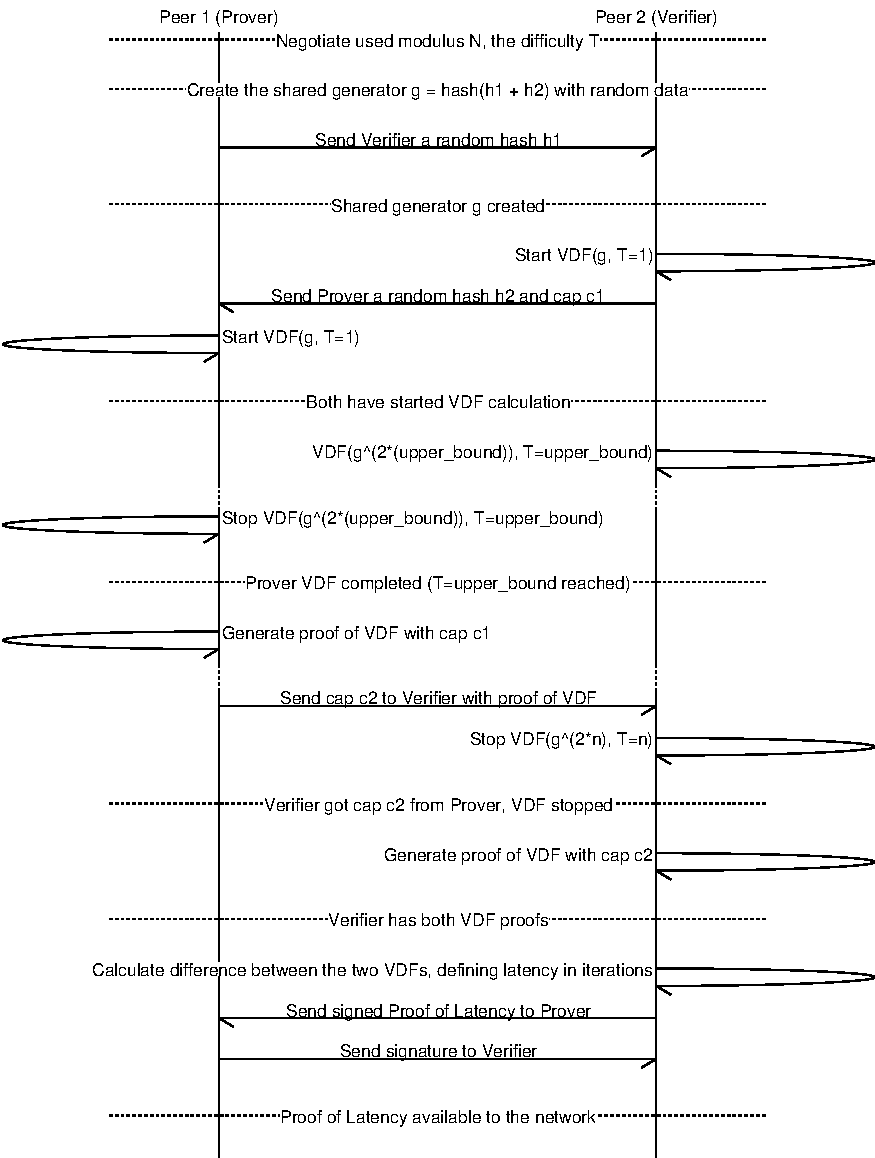
\includegraphics[width=\textwidth]{pictures/pol2_diagram-eps-converted-to.pdf}
	\caption{Distance bounding, Proof of Latency.}
	\label{PoL Diagram 2}
\end{figure}

In the setup, before the distance bounding, the prover and the verifier send their generator parts to themselves to construct a generator, or the starting point, for the VDF. Then, they both start calculating the same VDF independently. The prover then calculates the VDF up to a predefined threshold, and then sends the result at that threshold to the verifier, and starts calculating the proof. Proof is only sent after this, because since the VDFs the two parties calculate have the same input that was defined at roughly the same time, the parties can be sure that the result couldn't have been computed beforehand. The verifier stops its own calculation upon receiving the prover's result, and generates a proof of its own VDF. Then, it waits until it receives the proof from the verifier and then calculates the absolute difference between the amount of iterations between its own VDF and the prover's.

Since calculating a VDF is relatively fast for modern processors, a VDF over as little as a few milliseconds of time can be a valid way of measuring latency. Still, without an ASIC chip for calculating VDFs faster than any other available processor, these protocols are also a measurement of processing performance. This might introduce an unfortunate barrier for entry for mobile and IoT devices. If used to optimize a P2P network, the resulting network topology would result in a gradient that is defined by geographical location and the similarity in performance. This means that connectedness between mobile and IoT devices is going to be better than between devices that have a huge performance difference. Local performant devices would optimally serve as bridges between the localized clusters.

The distance bounding algorithm can be thought of as a state machine, or in fact, two state machines running in parallel.

\begin{figure}[htp]

	\centering
	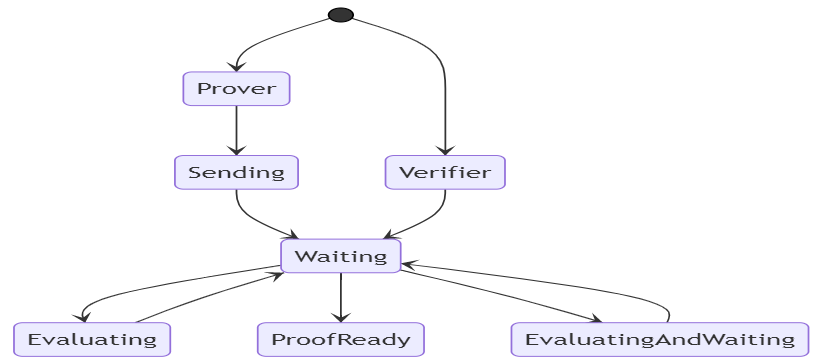
\includegraphics[width=.3\textwidth]{pictures/mermaid-diagram-20210505012010.png}\hfill
	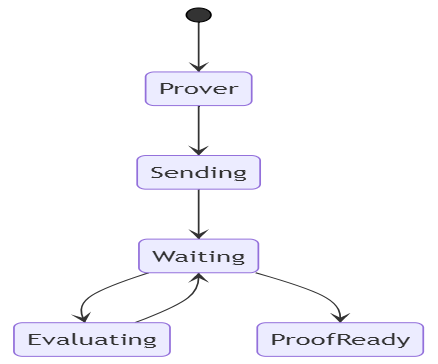
\includegraphics[width=.3\textwidth]{pictures/mermaid-diagram-20210505014229.png}\hfill
	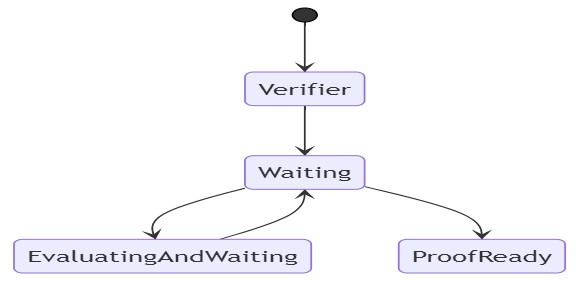
\includegraphics[width=.3\textwidth]{pictures/mermaid-diagram-20210505015712.png}

	\caption{Possible states for the state machines.}
	\label{Protocol States}

\end{figure}

\subsection{Finalizing}
% TODO: Go over a imagined case of advertising the proofs to other peers on a network
\section{Use Cases}
\begin{figure}
	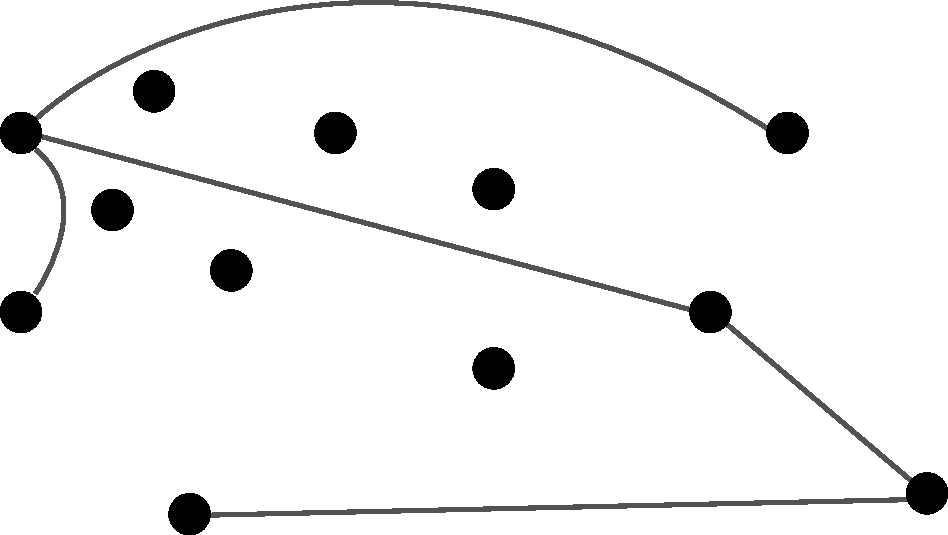
\includegraphics[width=\textwidth]{pictures/random_routing.pdf}
	\caption{Example suboptimal routes achieved by randomly selecting peers.}
	\label{Subobtimal Topology}
\end{figure}
Section 2.2 on peer-to-peer networking described some problems Proof of Latency is meant to help with. While peer-to-peer networking is an obvious area for Proof of Latency, the same protocol can be used also for computation performance benchmarking, VDF calculation using the latency proofs themselves, and to prove a geographical location. In the next sections I will describe these use cases more thoroughly.

\subsection{Dynamic P2P Routing}
The use case that drove me to begin working on Proof of Latency is an idea that there could be a trustless way for peers to tell other peers how much latency they have to other peers. In current P2P systems, if one peer were to tell you that it had a 10ms latency to another peer, there would be no quarantees of the 10ms latency holding true. If we could make a proof of that latency using cryptography, you could tell that the reported latency is true, and that some work has been done to calculate it. This kind of proof could also make eclipse attacks harder to accomplish by requiring a closer distance or more resources to reach a lower latency to the targeted peer.

Although DHTs like Kademlia do peer distribution basically at random based on identifier closeness, there are no guarantees that when a peer connects to the peers it has received from an another peer are also random, and thus the promise of random peer walk is lost. With Proof of Latency, new connections are formed in a hybrid manner together with a peer discovery mechanism that can provide protection against sybil attacks by introducing as random peers as possible, which helps in finding an approximate set of connected peers that are close to the possible minimum latency. Stochastic gradient descent works as a nice parallel from the machine learning field to describe randomness' use as an optimization tool.

\subsection{Benchmark Queries}
Like any time-lock puzzle~\cite{Mahmoody2013-zi}, the distance bounding part of Proof of Latency could be used to query for performance. Processor development might render that property less effective in the future, unless one were to measure parallel processing capability with multiple VDFs, for example. Parallel multiple VDFs have been thought of and tested before, but calculating multiple separate VDFs has not been useful in previously imagined use cases, since it doesn't serve as a measure of time, but performance.

Benchmark queries done with VDFs could serve as a part of a protocol in a distributed computation system. It would be very unfortunate to run large datasets against a data analysis model on a mobile phone, and it could be beneficial to prove that the peer that advertises its services can actually run the computation without hiccups.

There have been proposals for a VDF-as-a-function system~\cite{Devlin2020-qw}, in which less performant peers could query for a VDF calculation if they don't have the means to do so in a time frame small enough themselves. The FPGA based system is being tested right now on Amazon Web Services cloud platform. A benchmark query using PoL could also be a part of such a system to verify peers' ability to perform VDF calculations faster than the querying peer.

\subsection{VDF Calculation with Proved Latencies}
Assuming the soundness of the proofs created by Proof of Latency holds, given a VDF challenge with difficulty \(T\) the prover could craft a route of \(n\) peers that have the needed amount of PoL-measured latency (in VDF iterations) between them. Even a weaker device could then start a game of broken telephone with these peers that would guarantee sequential message passing by repeated hashing with signatures, and give the resulting signed response as a VDF to the verifier. Because of the precomputation that has been done to prove the individual latencies between the peers, one could prove that a received challenge has taken roughly \(T\) amount of sequential operations to solve by relaying it through a route of peers on the network. In such a network, VDFs would be first-class citizens and always available, equally for every participant of the network. This means that both computationally powerful and weak peers could equally take part in things that require a delay function to be evaluated and proven without either benefiting from the situation disproportionately.

\subsection{Proving Geographical Locations}
GPS coordinates or geohashes or any widely used geolocating method do not contain a proof of the reporter's proximity to the reported location. At first, I called Proof of Latency Proof of Proximity, but since it also measures processing power, I decided to go with latency instead, as there's many types of latencies that account for latency in P2P communication. Still, in roughly the same way as in dynamic P2P routing, a proof could be created that the prover is close to the verifier, and give or restrict access to resources based on this proof.

\section{Security Analysis}
Since Proof of Latency removes security quarantees by removing randomness from routing, some new attack vectors are introduced. Proof of Latency is not meant to be a one-stop shop towards a safer network, but rather an add-on to make the aforementioned use cases more efficient while still keeping security in mind. The following imagined attack vectors to create or advertize false proofs are a product of prior knowledge, research and the writer's thought process, and none have been tested out in practice, yet.
% TODO: More stuff on the basic security assumptions of the protocol. What are prior knowledge? Cite.

\subsection{Advertising Dishonest Peers and Proof Spoofing}
A malicious network participant can spawn an arbitrarily large number of new identities and network peers that are close-by in terms of latency, create multiple Proofs of Latency with them, and only advertise these peers to the rest of the network on their DHT. Two peers can also fake the proof if they co-operate by using VDFs they have already calculated and matched their outputs to be as close as possible.

Advertizing dishonest peers can be mitigated somewhat by requiring peers to renew their proofs regularly, using third party validators or a verifiable source of randomness, like a random beacon or a public timestamping service with signed requests. Also, trusted computing modules could be used to verify that the prover's software configuration has not been changed, removing most of the possibility for side channel attacks against using witnesses.

\subsection{Performance Matching}
The Proof of Latency protocol suffers from an issue, let's call it performance matching, which is a timing attack. Timing attacks are side-channel attacks against computer systems. Side-channel attacks utilize information from outer factors affecting the hardware and software the attacked program runs on. Timing attacks rely on gathering of timing data from the target.~\cite{noauthor_undated-mp} In performance matching, gathering data could be done by connecting to the targeted peer by another protocol or comparing existing proofs of latencies from all peers that have calculated their latency with the target.

Performance matching enables attackers to perform an eclipse attack on low-performance devices by matching the attacker's performance with the targeted mobile device so that it is as close as possible in the difference between iterations in PoL. This attack could result in a complete network split, as performance differences between devices make peers inaccessible to the other side of the performance spectrum, as network latencies can't compete with the computing power. There is a fundamental barrier for entry to this attack, which is that the attacker must have a more performant processor to calculate the VDF than the target. The malicious peer cannot performance match if its performance is worse or similar to the targeted peer, because of the race between them, without the target co-conspiring with the attacker.
% TODO: Mention the added security provided by vector commitments

\section{Reducing the Attack Vectors}
\subsection{Hiding Information of PoL Results}
If the publicized proof did not include both the VDF results and iterations, but just the iteration difference, an attacker would have less info on each peer. This would make attacking more difficult, requiring more queries and PoL runs on average before finding a vulnerable peer. This is more of an exploratory path that would need more research, but if you could create a proof of the latency and only broadcast the iteration difference between two peers, it would be more difficult to gather info about peers and their computing performance.

\subsection{Web of Trust}
There's also a possibility of introducing a web of trust in parallel to PoL to recognize and deny connections to malicious peers more effectively. An example of such a system is SybilLimit, which adds a construction called trusted routes to DHT based routing~\cite{Yu2008-xl}. I see that trusted routes in conjunction with Proof of Latency would be a great couple. The problem of advertising dishonest peers could also be tackled with a trust based system.

\subsection{Peer Scoring and Usage Optimizations}
Peer scoring is used regularly in P2P networks, and Proof of Latency serves as a peer scoring metric by itself, which can be used in various ways. To hinder eclipse attacks, connections to peers with the lowest latencies would be kept open for a longer time, even in the case of the peer not being online, and favoring new ephemeral connections that are farther. This would require the attacker to pursue multiple attack vectors at once to totally eclipse a peer.

% TODO: What about punishing peers if they advertize two squaring speeds for themselves without devalidating the old one?

\subsection{Using a Third Party Validator}
A way to make Proof of Latency more trustless is to introduce a randomly elected third party to the protocol. Since the soundness of the proof depends largely on the generator and its setup, the proof can be improved by requiring it to be salted\footnote{A value that gets added to data by contract before hashing.} by a random input from an unbiased party. This could be done by introducing a salt pool to which a group of PoL validators post random salts from which the PoL provers then pick randomly. The validators listen for usage of the salts they have generated, and upon receiving the Proof of Latency inspect if their salt has been used or not, and sign the proof if it is found to be correct.

% TODO: Using a Witness selection scheme based on random IDs in Kademlia which prevents sybil attacks because close-by identities are hard to create. Three-way creation of the proof with the witness providing a salt together with a measurement of the verifier's/prover's hash rate, or squarings per second

% TODO: Shuffling peer connections?

\subsection{Replicating the Vector Commitment}
% TODO: Publishing the vector commitment on chain or adding redundancy to "lock it in place" Sort of is locked already, because it's deterministic.

\chapter{Proof of Concept}
\label{Proof of Concept}
To test out the Proof of Latency, I wrote a software proof of concept in Rust. I picked Rust as a programming language of choice because it has good properties when it comes to cryptography and distributed computing. Since distributed computing, or any server program for that matter, uses some sort of concurrency to get non-blocking responses to requests they receive, the programmer has to worry about race conditions, with most systems programming languages. Rust is different, however, as when a Rust program has been compiled in the default "safe" compiler setting, a data race where two or more threads try to access a shared memory resource at the same time is simply impossible to achieve~\cite{The_Rust_Project_Developers2018-xh}. Also, as it is a compiled language without a garbage collector, and with lots of optimization in the compiler, Rust has good baseline performance, on par with C or C++~\cite{Howarth2020-zc}. Rust has seen a surge of interest in the last few years, and it is used in many projects in production, notably in embedded and distributed computing, because of Rust's modern build tooling and robustness.

William Borgeaud's blog post~\cite{Borgeaud2019-wk} from November 2019 was the first reference I encountered that described VDFs in terms familiar to software engineers. The blog post and it's accompanying code~\cite{Borgeaud2019-wk}, that also happened to be in Rust, helped me bootstrap the project.

In the implementation of the VDF protocol, the computations need to run asynchronously, on separate threads. There needs to be a separate task for listening to the other party's input, and preferably, a way to test the protocol locally without networking. The PoL protocol needs a VDF such that the prover's calculation can be ran indefinitely and then ended abruptly by a received "cap", a prime number from the verifier. No previous VDF library seemed to have this option, because the difficulty parameter \(T\) is usually predetermined, which is not the case for the prover in Proof of Latency.

The code is structured as follows: Runnable binary demo and the reusable library it uses resides in the top crate. They depend on subcrates that individually provide functionalities like VDF calculation and vector commitments.

\begin{figure}
	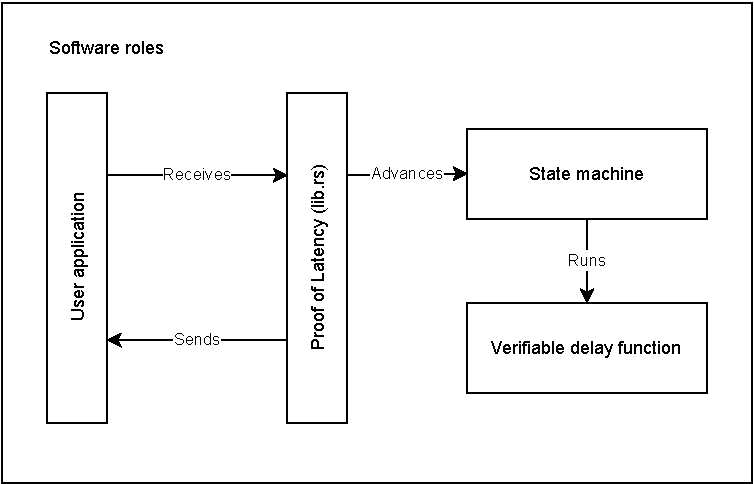
\includegraphics[width=\textwidth]{pictures/PoL_software_roles.pdf}
	\caption{Software roles}
	\label{software_roles}
\end{figure}

The protocol is implemented as a state machine, which helps checking the protocol with model checkers, like TLA+. % CITE
 The protocol implementation uses variable names derived from the protocol description in fig % CITE
 , with slight adaptation from mathematical notation to a more semantic approach.

\begin{figure}
	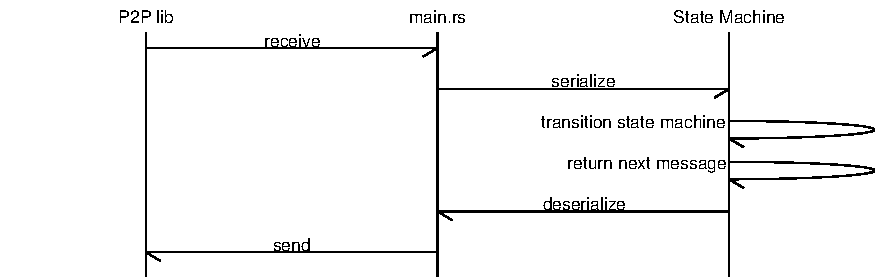
\includegraphics[width=\textwidth]{pictures/message_flow-eps-converted-to.pdf}
	\caption{Usage of Proof of Latency as a library in a P2P context.}
	\label{message_flow}
\end{figure}

The following is a code example of the threaded valuation part of a VDF inside Proof of Latency, containing evaluation stop logic for both the prover and the verifier:
\lstinputlisting[language=Rust, float, frame=lines, breaklines=true, caption=VDF iteration logic]{./parts/code/vdfiteration.rs}

The following is a code example of the proof generation of a VDF:
\begin{listing}
	\inputminted
	[
		frame=lines,
		framesep=2mm,
		baselinestretch=1.2,
		fontsize=\footnotesize,
		tabsize=2,
	]
	{Rust}{./parts/code/proofgeneration.rs}
	\caption{VDF proof generation}
	\label{lst:proofgeneration.rs}
\end{listing}

The following is a code example of the verification of a VDF proof:
\begin{listing}
	\inputminted
	[
		frame=lines,
		framesep=2mm,
		baselinestretch=1.2,
		fontsize=\footnotesize,
		tabsize=2,
	]
	{Rust}{./parts/code/verifyvdf.rs}
	\caption{VDF proof verification}
	\label{lst:verifyvdf.rs}
\end{listing}

The proof of concept is implemented as a library, so that it can be imported and used in other projects.

% TODO: TESTS!

\section{Tests}
To gain assurance of the correctness of the VDF calculations I wrote unit tests for the VDF evaluation, proof generation and verification. To further ensure the soundness of the protocol, I added integration tests for Proof of Latency with separate, asynchronous threads for each execution. The tests reside in same files as the program code itself. The Rust standard library has good support for unit testing so that no separate library was needed.

In addition to regular unit tests with predefined input, I experimented with property testing. Property testing is a term that belongs somewhere between fuzzing\footnote{Testing systems against a randomized, high volume of input.} and unit tests. Otherwise it functions like regular unit tests, but it adds generated input into the equation. By adding generated, sometimes randomized input, one can check more thoroughly for edge cases. While being effective in recognizing some unexpected bugs, it still has a way to go when compared to formal verification, which is a testing method that aims to define a system with mathematical proofs, verifying that the output should always, apart from hardware issues, be correct according to the specification.

%\subsection{End to End Tests}
%To test the whole demo out in a simulated P2P setting I used Protocol Labs' Testground software. It is a tool to simulate a network with thousands of peers on one machine.
%TODO: add more stuff after getting the p2p to work
